%%%%%%%%%%%%%%%%%%%%%%%%%%%%%%%%%%%%%%%%%
% fphw Assignment
% LaTeX Template
% Version 1.0 (27/04/2019)
%
% This template originates from:
% https://www.LaTeXTemplates.com
%
% Authors:
% Class by Felipe Portales-Oliva (f.portales.oliva@gmail.com) with template 
% content and modifications by Vel (vel@LaTeXTemplates.com)
%
% Template (this file) License:
% CC BY-NC-SA 3.0 (http://creativecommons.org/licenses/by-nc-sa/3.0/)
%
%%%%%%%%%%%%%%%%%%%%%%%%%%%%%%%%%%%%%%%%%

%----------------------------------------------------------------------------------------
%	PACKAGES AND OTHER DOCUMENT CONFIGURATIONS
%----------------------------------------------------------------------------------------

\documentclass[
	12pt, % Default font size, values between 10pt-12pt are allowed
	%letterpaper, % Uncomment for US letter paper size
	spanish, % Uncomment for Spanish
]{fphw}

\usepackage{setspace}
%\singlespacing
\onehalfspacing
%\doublespacing

% Template-specific packages
\usepackage[utf8]{inputenc} % Required for inputting international characters
\usepackage[T1]{fontenc} % Output font encoding for international characters
\usepackage{mathpazo} % Use the Palatino font
\usepackage{hyperref}
\hypersetup{
    unicode=false,          % non-Latin characters in Acrobat’s bookmarks
    pdftoolbar=true,        % show Acrobat’s toolbar?
    pdfmenubar=true,        % show Acrobat’s menu?
    pdffitwindow=false,     % window fit to page when opened
    pdfstartview={FitH},    % fits the width of the page to the window
    pdftitle={My title},    % title
    pdfauthor={Author},     % author
    pdfsubject={Subject},   % subject of the document
    pdfcreator={Creator},   % creator of the document
    pdfproducer={Producer}, % producer of the document
    pdfkeywords={keyword1, key2, key3}, % list of keywords
    pdfnewwindow=true,      % links in new PDF window
    colorlinks=true,       % false: boxed links; true: colored links
    linkcolor=red,          % color of internal links (change box color with linkbordercolor)
    citecolor=green,        % color of links to bibliography
    filecolor=magenta,      % color of file links
    urlcolor=cyan           % color of external links
}
\usepackage{caption}
%\captionsetup{labelformat=empty}


\usepackage{graphicx} % Required for including images

\usepackage{booktabs} % Required for better horizontal rules in tables

\usepackage{listings} % Required for insertion of code

\usepackage{enumerate} % To modify the enumerate environment

\usepackage{amsmath}

%----------------------------------------------------------------------------------------
%	ASSIGNMENT INFORMATION
%----------------------------------------------------------------------------------------

\title{Integridad Visual} % Assignment title

\author{Juan Andres Knebel} % Student name

\date{\today} % Due date

\institute{Universidad de Buenos Aires \\ Maestría en Explotación de Datos y Descubrimiento del Conocimiento} % Institute or school name

\class{Visualización de la información - Trabajo práctico \#2} % Course or class name

%\professor{Dr. Albert Einstein} % Professor or teacher in charge of the assignment

%----------------------------------------------------------------------------------------

\begin{document}

\maketitle % Output the assignment title, created automatically using the information in the custom commands above

%----------------------------------------------------------------------------------------
%	ASSIGNMENT CONTENT
%----------------------------------------------------------------------------------------

\section*{Ejemplos de gráficas}

\subsection*{Primera elección}

\textit{Un gráfico está distorsionado si la representación visual que presenta no se condice con la representación numérica.}

\begin{figure}[ht]
\begin{center}
	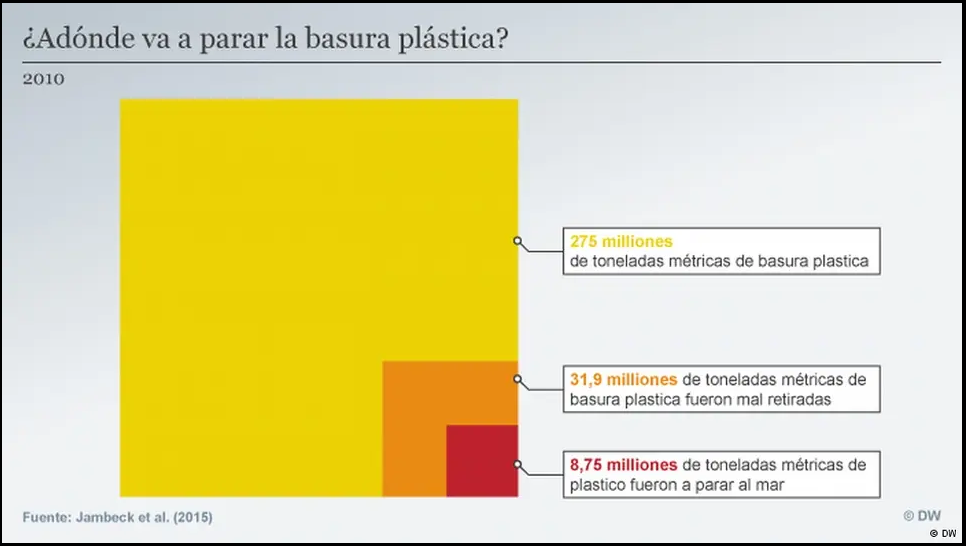
\includegraphics[width=1\columnwidth,keepaspectratio]{lanacion-plasticos.png}
	\caption*{Fuente: \href{https://www.lanacion.com.ar/sociedad/6-graficos-para-entender-el-problema-del-plastico-nid1968639}{Diario La Nación}}
\end{center}
\end{figure}

$$ \textbf{Factor de Mentira}\ =\ \dfrac{proporci\acute on\ en\ el\ gr\acute afico}{proporci\acute on\ en\ los\ datos} $$

Se muestra un incremento que va desde los 8.75 millones hasta los 275 millones, o lo que es lo mismo una variación cercana al 3042\%.

$$ \dfrac{275 - 8.75}{8.75} \times 100  \approx 3042$$

El lado del cuadrado que representa los 275 millones tiene un longitud de 10.5 cm, siendo su área de 110.25 $cm^{2}$.

El lado del cuadrado correspondiente a los 8.75 millones es de 2.9 cm, resultando su área en 8.41 $cm^{2}$. Dando como resultado una variación aproximada del 1210\%

$$ \dfrac{110.25 - 8.41}{8.41} \times 100  \approx 1210$$


$$ \textbf{Factor de Mentira}\ = \dfrac{1210}{3042} \approx \boxed{0.39} $$

Siendo que el factor de mentira es de $\textit{0.39} < 0.95$, se puede decir que el gráfico no está representando los datos adecuadamente. También se puede ver que como $log(0.39) < 0$ entonces se está incurriendo en un error por reducción.

\newpage
\subsection*{Segunda elección}

\textit{En las series de tiempo monetarias, casi siempre es mejor usar unidades estandarizadas en lugar de nominales.}

\begin{figure}[ht]
\begin{center}
	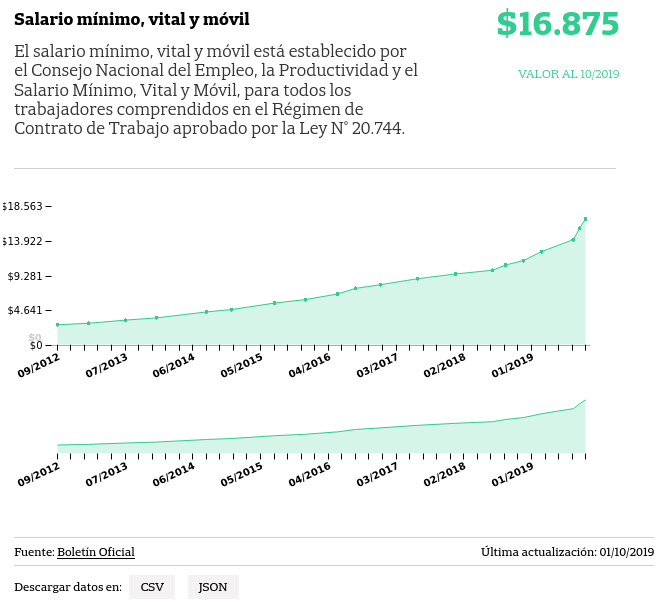
\includegraphics[width=0.75\columnwidth,keepaspectratio]{lanacion-salirio-minimo.png}
	\caption*{Fuente: \href{https://www.lanacion.com.ar}{Diario La Nación}}
\end{center}
\end{figure}

Se muestra la variación del salario mínimo, vital y móvil a través de los últimos 7 años en la Argentina utilizando el valor nominal del peso argentino. Teneindo en cuenta que en los últimos 7 años el país pasó y pasa por períodos de inflación por encima del 20\% y fuertes devaluaciones con respecto al dólar, el gráfico presentado no aporta nada por si mismo.

\newpage
%----------------------------------------------------------------------------------------

\section*{La peor visualización del mundo}

Para realizar la peor visualización se obtuvo un data set que contiene los datos acerca de robos de autos durante el mes de abril de 2020. Fuente: \href{https://datos.gob.ar/dataset/justicia-robos-recuperos-autos/archivo/justicia_c46fe6e0-6d29-4427-907e-d37c0d7c32c4}{Portal de datos de argentina}.

\begin{figure}[ht]
\begin{center}
	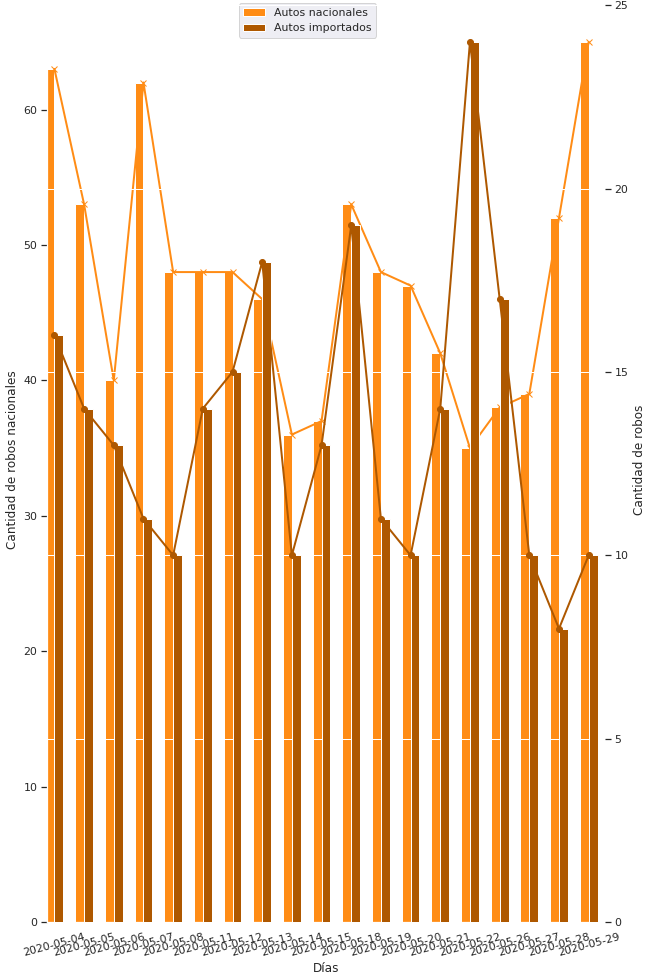
\includegraphics[width=0.7\columnwidth,keepaspectratio]{peor_grafica-mod.png}
	\caption*{Robos de auto por día hábil}
\end{center}
\end{figure}

En el gráfico propuesto se puede ver la longitud de las barras representan cantidades completamentes diferentes tanto para los autos nacionales como para los importados. En los autos nacionales 23.2 cm. de una barra equivale a 65 autos, mientras que para los importados esa misma distancia corresponde a 24 autos. La cantidad tampoco se encuentra normalizada sobre el total del parque automotor, por lo que tampoco se podría distinguir si se roban más autos nacionales o no.

La elección de colores es confusa ya que si bien se pude diferenciar uno del otro, resulta muy dificíl mirar el gráfico como un todo y poder sacar algún tipo de conclusión. El agregado de las líneas para marcar los descensos y ascensos tampoco ayudan a la interpretación. Las leyendas de las fechas sobre el eje x si bien se pueden leer estan dispuestas de una manera que confunden la pertenencia de las barras a las fechas. Por último sobre el eje y del lado izquierdo se indica que es la cantidad de autos robados que pertenecen solo a los autos nacionaeles, del lado derecho en cambio, hay que concluir que se trata de los autos importados.

El gráfico también se realizó mucho más alargado que ancho para mostrar la vertiginosidad en las cantidades.

Principios que no se cumplen en este gráfico son:
\begin{itemize}
	\item \textit{Debemos visualizar la variación en los datos, no en el diseño}.
	\item \textit{La dimensión de los datos no puede ser superada por la dimensión del gráfico}.
	\item \textit{Los gráficos no deben sacar los datos de contexto}.
\end{itemize}

\end{document}
